\subsection{Beschreibung HMI - Main}
\label{kap:ClientGraphProgramm}
Die HMI gliedert sich in mehrere Bereiche, in denen verschiedene Funktionalit�ten bereitgestellt werden. Diese finden im folgenden Abschnitt Erl�uterung. 

\begin{figure}[H]
\centering
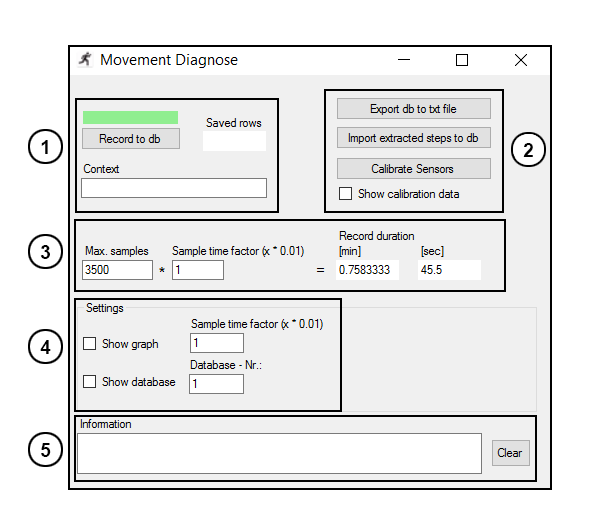
\includegraphics[width=1.0\linewidth]{03_Grafiken/Messsystem/ClientGraph_Gui}
\caption[Client Graph HMI]{Client Graph HMI}
\label{fig:clientgraphgui}
\end{figure}

\begin{enumerate}
	\item \textbf{Aufnahme / Import, Export / Visualisierung} \\
	Der gr�ne Balken dient als Indikator, ob Messwerte empfangen werden (gr�n: Messung kann gestartet werden, rot: Es werden keine Daten empfangen).\\
	Durch das Bet�tigen des Buttons \textit{Record to db} wird eine Messung gestartet bis diese abgebrochen oder die max. Anzahl an Samples erreicht wird.\\
	Das Label \textit{Saved rows} zeigt die aktuelle Anzahl aufgenommener Messwerte an.\\
	Durch das Bet�tigen des Buttons \textit{Upload steps} erfolgt das Importieren einer CSV-Datei (ohne �berschrift) in das Programm, welches diese dann in eine externe SQL-Datenbank hochl�dt.
	Im Textfeld \textit{db name} muss die Bezeichnung der Tabelle eingegeben werden, in welche die Messwerte hochgeladen werden sollen.

	Mit dem Bet�tigen des Buttons \textit{Export...} erfolgt das Exportieren der erfassten Sensordaten in eine CSV-Datei. Jeder Sensor generiert eine eigene Datei mit dem unter \textit{Context} angegebenen Namen.\\
	Diese Funktion soll in der n�chsten Version automatisiert im Hintergrund stattfinden, sodass es, zum Hochladen in die externe Datenbank, nur ein Button exisitert.
	
	Durch das Setzen des H�kchens bei \textit{Show graph} werden die Sensorwerte visualisiert. Durch das Setzen des H�kchens bei \textit{Show database} werden die Eintr�ge der Datenbank dargestellt.
		
	\item \textbf{Settings}\\
	In das Textfeld \textit{Max. samples} wird die aufzunehmende Anzahl an Messwerten eingetragen. Danach stoppt die Messung automatisch. Standardm��ig sind 3500 Samples eingetragen, da bei einer zu gro�en Anzahl eine \textit{Out of memory Exception} geworfen wird.
		
	Durch das Bet�tigen des Buttons \textit{Calibrate Sensors} erfolgt das Kalibrieren aller Sensoren (s. Beschreibung in \ref{kap:Erfassungsprogramm}). Durch das Setzen des H�kchens \textit{Show...} erfolgt das Darstellen der kalibrierten Sensorwerte.
	
	F�r das Exportieren der Messwerte in eine Text-Datei kann ein Dateiname angegeben werden. Bleibt dieses Feld leer, so lautet der Dateiname: noname\_x (x steht f�r die Zahl des Sensors).
		
	\item \textbf{Information}\\
	In dem Textfeld erfolgt das Darstellen wichtiger Systemereignisse (z.B. Fehler), die durch das Bet�tigen des Buttons \textit{Clear} gel�scht werden k�nnen.
\end{enumerate}

